% !TEX root = ../paper.tex

\section{Method}

\subsection{Problem Formulation}

We study infrared-visible registration as a scene-level alignment task. For each scene, the input is
a set of paired RGB and thermal UAV frames
$S = \{(I_i^R, I_i^T)\}_{i=1}^N$, where viewpoint variation, cross-resolution sensing, thermal
appearance changes, and day/night conditions make individual frame estimates uneven in quality. The
goal is to recover a thermal-to-RGB homography that remains reliable at the scene level, with the
canonical output retained when the evidence satisfies the reliability criterion.

This formulation turns registration from a single best-pair problem into a multi-frame reliability
optimization problem. In our setting, many scenes already contain usable pairwise correspondences,
but the central challenge is to convert uneven frame-level estimates into a transform that is
geometrically stable, internally consistent, and acceptable under a reliability-aware criterion.
For a selected frame pair, the thermal-to-RGB evidence is represented as a homography
$H_i \in \mathbb{R}^{3 \times 3}$ acting on homogeneous image coordinates,
\begin{equation}
\tilde{\mathbf{p}}^{R}_{ij} \sim H_i \tilde{\mathbf{p}}^{T}_{ij},
\qquad
H_i = \arg\min_H \sum_{j \in \mathcal{I}_i}
\rho\!\left(\left\|\pi(H\tilde{\mathbf{p}}^{T}_{ij}) -
\mathbf{p}^{R}_{ij}\right\|_2^2\right),
\label{eq:pairwise_homography}
\end{equation}
where $\mathcal{I}_i$ denotes the inlier set selected by robust fitting, $\pi(\cdot)$ converts a
homogeneous coordinate to image coordinates, and $\rho(\cdot)$ is the robust estimator loss. The
scene-level problem is then to estimate a consensus transform $\bar{H}_S$ from uneven evidence
$\{H_i\}$ and decide whether it should be retained as an alignment product.

\begin{figure}[t]
\centering
\makebox[\textwidth][c]{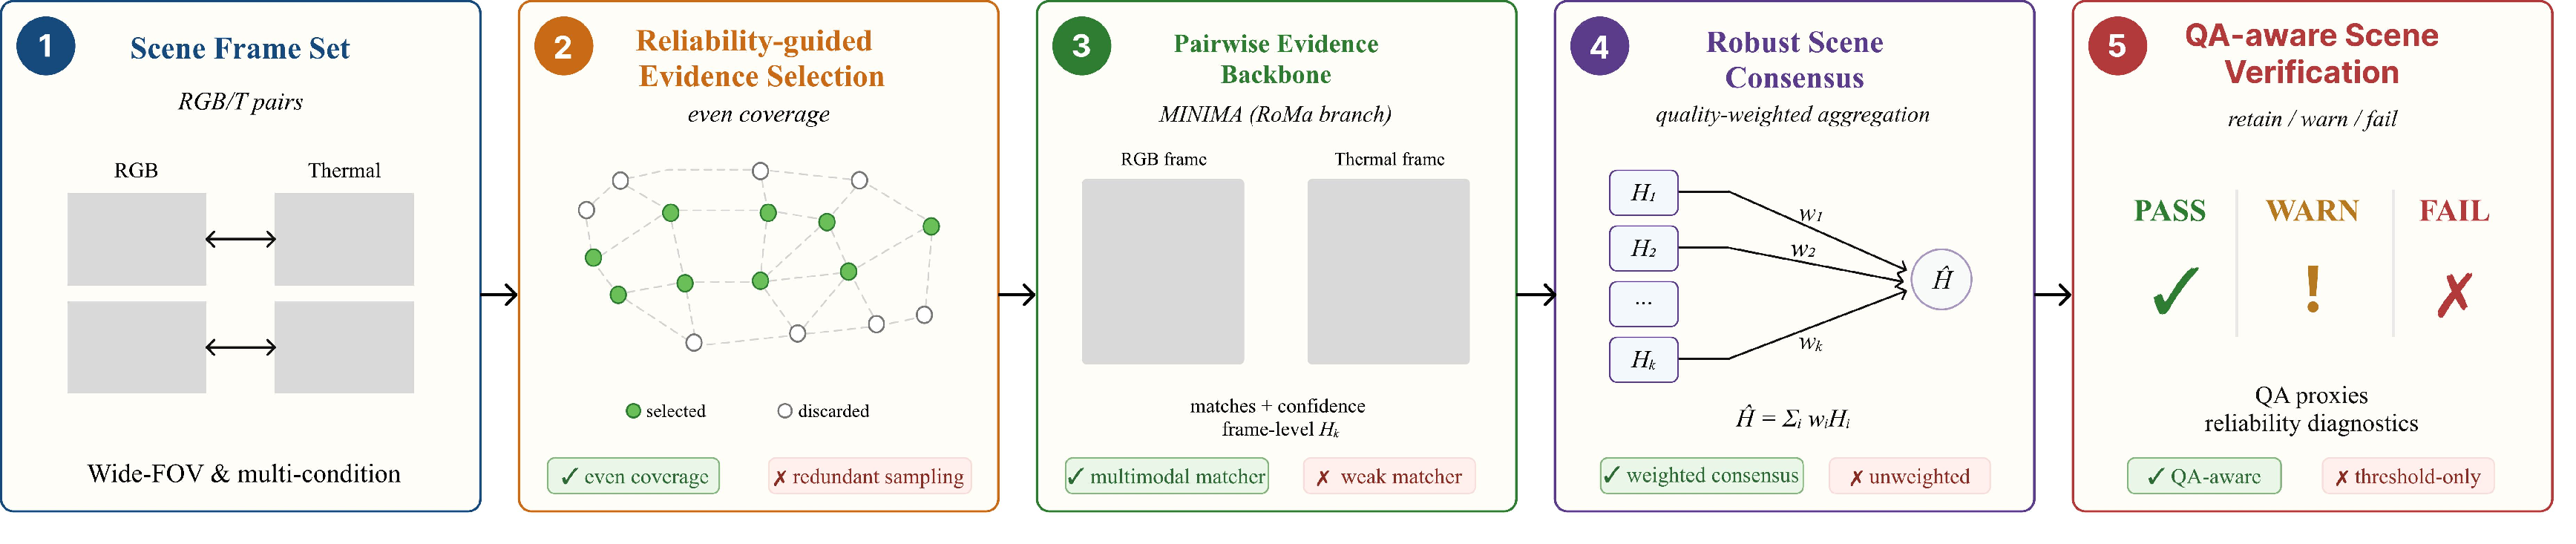
\includegraphics[width=1.35\textwidth]{figures/fig_method_pipeline.pdf}}
\caption{Overview of UAV-TAlign. The framework builds on strong pairwise matching, but
makes the final decision at the scene level through reliability-guided evidence selection, robust
scene consensus, and QA-aware verification.}
\label{fig:method_pipeline}
\end{figure}

\subsection{Pairwise Evidence Backbone}

UAV-TAlign uses a strong off-the-shelf multimodal matcher as its pairwise evidence generator. Our
implementation uses the MINIMA family with the RoMa branch as the default backend, while the
rest of the pipeline remains agnostic to the exact pairwise matcher
\cite{edstedt2024roma,ren2025minima}.

\subsection{Reliability-Guided Evidence Selection}

At the scene level, UAV-TAlign prioritizes the most informative frame evidence before expanding the
support set. It uses a progressive evidence schedule that expands with scene size and can cover all
frames when needed. This reliability-guided policy allows the framework to stop when a compact
subset already yields a stable consensus, while still escalating to broader evidence when the scene
benefits from more support.

Within each stage, representative frames are selected with deterministic evenly distributed
sampling by default. This default policy is used for reproducibility and stable scene coverage. A
random-selection variant is reserved for sensitivity analysis and is reported separately.

\subsection{Quality-Weighted Frame Geometry}

For each selected frame pair, the matcher produces cross-modal correspondences that are filtered
into a frame-level homography estimate. UAV-TAlign evaluates each frame using
standard geometric statistics, including the number of matches, the number of inliers, inlier
ratio, reprojection error, and spatial coverage. A frame enters the global candidate pool only when
it passes a geometry-quality gate on these statistics. The overall geometric treatment remains rooted
in standard homography estimation and robust fitting practice
\cite{hartley2004multiple,fischler1981ransac,barath2019magsac,barath2020magsacpp}.

Beyond a binary accept/reject decision, the pipeline assigns each accepted frame a quality score so
that better-supported homographies receive more influence during scene aggregation. The score is a
weighted combination of inlier ratio, spatial coverage, reprojection quality, matcher confidence,
and inlier count. This keeps the scene-level estimate from being dominated by low-support frames
that only marginally satisfy the frame-level gate.
In normalized form, the frame quality weight is written as
\begin{equation}
q_i =
\alpha_r \phi(r_i) +
\alpha_c \phi(c_i) +
\alpha_e \phi(e_i) +
\alpha_m \phi(m_i) +
\alpha_n \phi(n_i),
\qquad
\sum_k \alpha_k = 1,\ \alpha_k \ge 0,
\label{eq:frame_quality}
\end{equation}
where $r_i$ is inlier ratio, $c_i$ is spatial coverage, $e_i$ is reprojection quality, $m_i$ is
matcher confidence, $n_i$ is inlier support, and $\phi(\cdot)$ maps each diagnostic into a
consistent reliability direction. The weights are fixed by the evaluation protocol and are not
learned from UAV-TAlign-12K.

\subsection{Robust Scene Consensus}

Once enough frame-level homographies have been accepted, UAV-TAlign forms a robust scene consensus.
Homographies are mapped into parameter space, centered with a median reference, and filtered by a
median-absolute-deviation rule to suppress unstable estimates before weighted averaging. The
retained homographies are then combined using the frame quality scores defined above.
Let $\mathbf{h}_i$ be the scale-normalized vector form of $H_i$. The consensus set is
\begin{equation}
\mathcal{C}_S =
\left\{i \in \mathcal{A}_S:
\left\|\mathbf{h}_i - \operatorname{median}_{j \in \mathcal{A}_S}(\mathbf{h}_j)\right\|_1
\le \tau_{\mathrm{mad}}\,\operatorname{MAD}(\{\mathbf{h}_j\}_{j \in \mathcal{A}_S})\right\},
\label{eq:consensus_set}
\end{equation}
where $\mathcal{A}_S$ is the accepted-frame set before robust consensus. The scene transform is
then obtained by quality-weighted aggregation,
\begin{equation}
\bar{\mathbf{h}}_S =
\frac{\sum_{i \in \mathcal{C}_S} q_i \mathbf{h}_i}
{\sum_{i \in \mathcal{C}_S} q_i},
\qquad
\bar{H}_S = \operatorname{mat}(\bar{\mathbf{h}}_S).
\label{eq:scene_consensus}
\end{equation}

The pipeline records stability diagnostics around the aggregate transform, including homography
dispersion relative to the aggregate and the ratio of robustly rejected frame-level estimates.
These diagnostics connect consensus formation with the final QA-aware decision.

\subsection{QA-Aware Scene Verification}

The final decision integrates match availability with scene-level reliability evidence. UAV-TAlign
evaluates the optimized scene-level transform against a label-free QA summary computed on
representative frames. The QA summary uses cross-modal proxy signals such as edge-overlap
improvement, gradient-NCC improvement, the ratio of improved frames, and the count of severe
relative outliers. It also retains scene-level match and stability statistics such as accepted-frame
ratio, mean inlier ratio, mean reprojection error, spatial coverage, dispersion relative to the
aggregate transform, and the robust reject ratio.

The canonical decision uses a baseline-aware verification rule. A scene is retained when
accepted-frame statistics remain strong, the aggregated homography is stable, severe
baseline-relative outliers remain controlled, and the transform improves gradient-based alignment
beyond configured floors. This final verification step gives UAV-TAlign its scene-level character:
the framework prioritizes retained scene-level usability over unconditional scene acceptance.
For operating-profile visualization, the same diagnostics are summarized by a non-trained
reliability score,
\begin{equation}
\begin{aligned}
R(S) ={}&
\beta_a A_S +
\beta_o (1-O_S) +
\beta_d (1-D_S) \\
&+
\beta_e \Delta E_S +
\beta_g \Delta G_S +
\beta_{\gamma} \Gamma_S,
\qquad
\sum_k \beta_k = 1 .
\end{aligned}
\label{eq:reliability_score}
\end{equation}
where $A_S$ is accepted-frame support, $O_S$ is severe baseline-relative outlier ratio, $D_S$ is
homography dispersion, $\Delta E_S$ and $\Delta G_S$ are edge and gradient improvement proxies,
and $\Gamma_S$ collects geometry diagnostics. The strict canonical gate remains a thresholded
decision on the underlying diagnostics,
\begin{equation}
y_S =
\mathbb{1}\!\left[
A_S \ge a_{\min},\ O_S \le o_{\max},\ D_S \le d_{\max},
\Delta G_S \ge g_{\min},\ \Gamma_S \in \mathcal{G}
\right].
\label{eq:canonical_gate}
\end{equation}
Thus $R(S)$ ranks scenes for risk-coverage analysis, while $y_S$ defines the retained canonical
alignment products reported in the main result.
